\chapter{Análisis de Resultados}
\label{chap:analisis-resultados}

Este capítulo presenta el análisis de los resultados obtenidos en la comparación entre el Algoritmo Genético (AG) y la heurística clásica \textit{Shortest Processing Time} (SPT). El objetivo es evaluar el desempeño de ambos métodos bajo condiciones realistas del taller, utilizando métricas relevantes para la programación diaria de tareas y considerando indicadores exclusivamente operativos.

El análisis combina una perspectiva técnica—basada en métricas cuantitativas, comportamiento estadístico de las soluciones y eficiencia algorítmica—con una interpretación industrial orientada a la toma de decisiones.

% -------------------------------------------------------------------
\section{Comparación Detallada AG vs SPT}
\subsection{Descripción general de los resultados}

Los promedios generales se encuentran en la Tabla~\ref{tab:comparacion-metricas} del Capítulo~\ref{chap:ejecucion-obtencion-resultados}. A partir de esos valores se observa que ambos métodos ejecutan, en promedio, la misma cantidad de tareas y rechazan un número equivalente; sin embargo, el AG obtiene un makespan significativamente menor y logra un mejor balance entre operarios, lo cual sugiere cronogramas más estructurados y eficientes.

El makespan promedio informado para el AG es 157.37 unidades de tiempo y el del SPT asciende a 186.53, es decir, una reducción cercana al 15.6\%. De manera similar, la desviación estándar de carga pasa de 35.11 (SPT) a 30.10 (AG), lo que equivale a una disminución del 14.3\%. Estas reducciones simultáneas indican que el AG concentra la misma carga total en un horizonte más compacto y con menor dispersión entre operarios.

% -------------------------------------------------------------------
\subsection{Análisis de distribución}

A continuación se presentan las distribuciones de desempeño para las métricas más relevantes. Según corresponda, las figuras se agrupan en pares para facilitar la comparación visual entre algoritmos.

% --- Figuras 1 y 2: Ejecución y rechazo ---
\begin{figure}[H]
\centering
\begin{subfigure}{0.45\textwidth}
    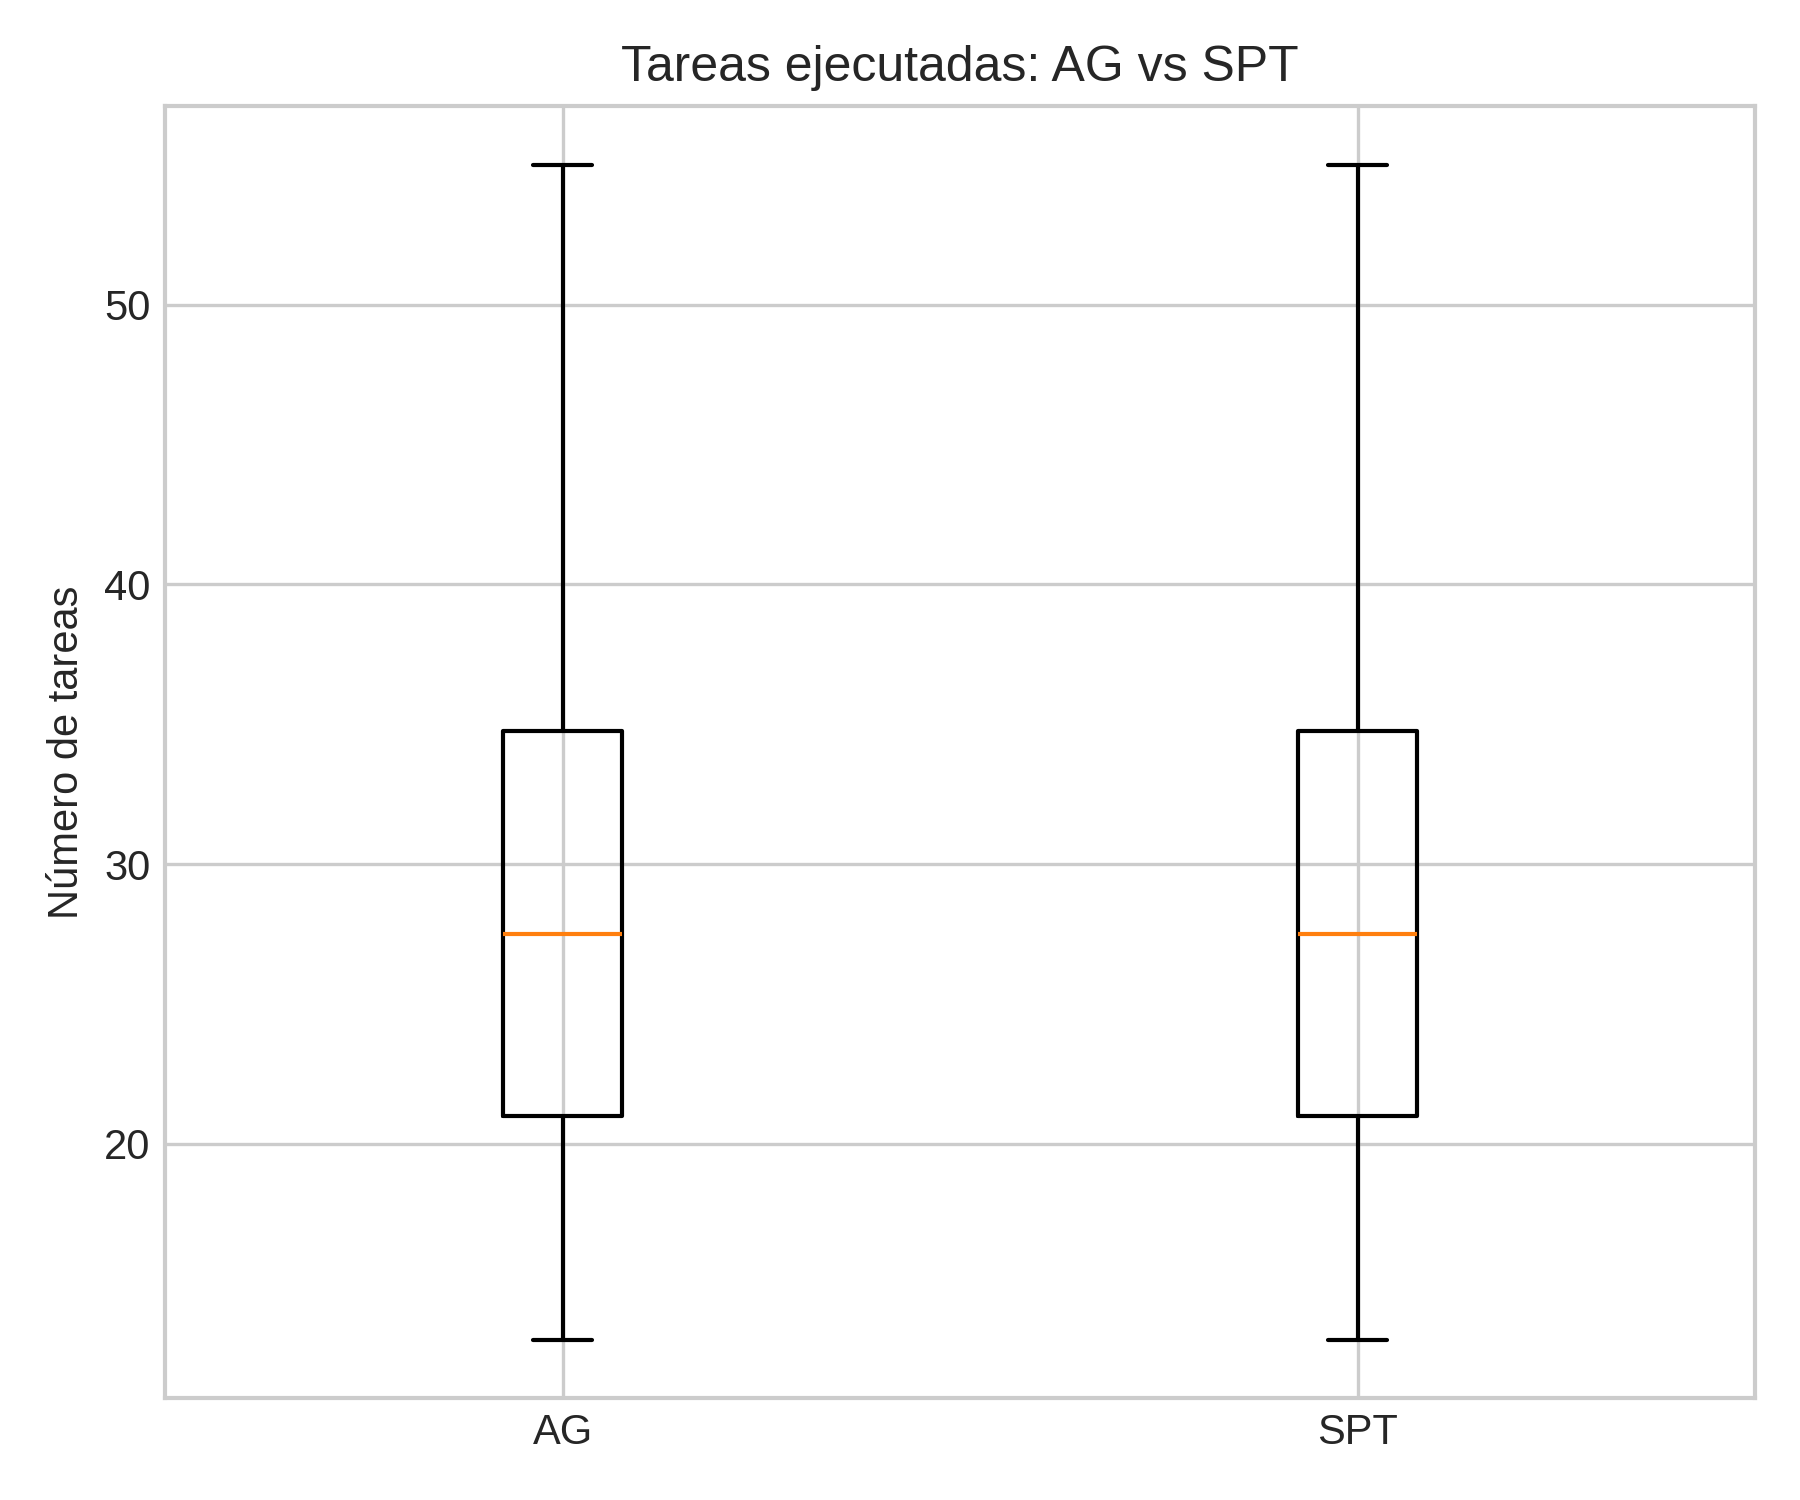
\includegraphics[width=\linewidth]{figures/tareas_ejecutadas.png}
    \caption{Tareas ejecutadas}
\end{subfigure}
\begin{subfigure}{0.45\textwidth}
    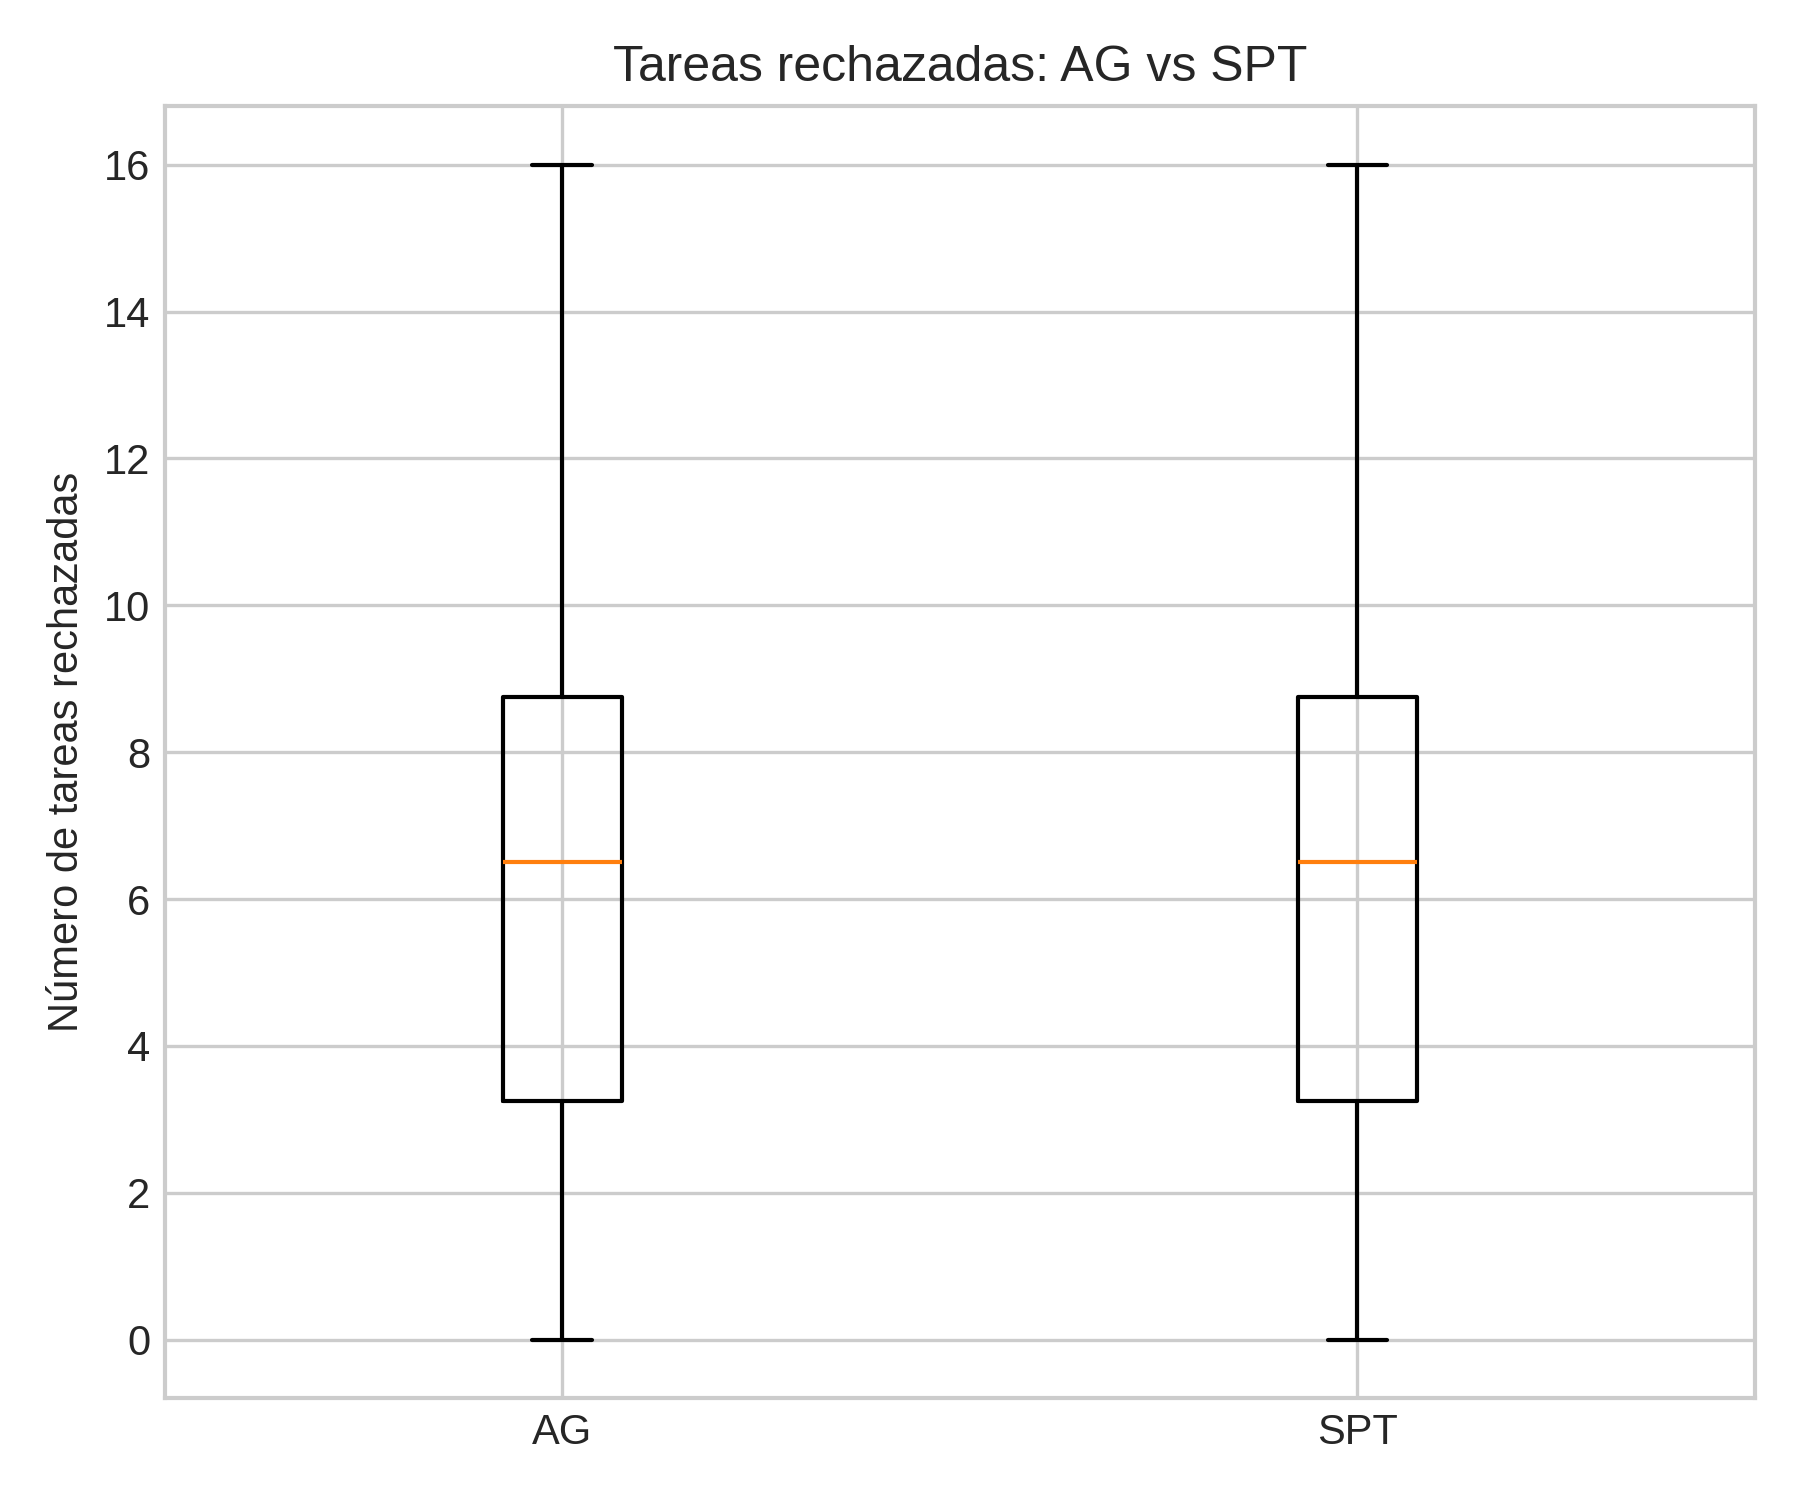
\includegraphics[width=\linewidth]{figures/tareas_rechazadas.png}
    \caption{Tareas rechazadas}
\end{subfigure}
\caption{Distribución comparativa de tareas ejecutadas y rechazadas.}
\label{fig:tareas-ejecutadas-rechazadas}
\end{figure}

Las distribuciones confirman que no existe una diferencia sistemática entre AG y SPT en cuanto al número de tareas completadas. Ambas técnicas logran niveles similares de factibilidad bajo las mismas restricciones del simulador.

% -------------------------------------------------------------------
\subsection{Tareas ejecutadas y rechazadas}
Aunque los promedios son iguales, la variabilidad es distinta: el AG presenta colas más compactas en sus distribuciones, lo que indica mayor estabilidad entre instancias. Desde la perspectiva del taller, esto significa cronogramas más predecibles y menor sensibilidad a la estructura de cada día de trabajo.

Las tareas rechazadas también muestran comportamientos equivalentes en promedio, aunque con ligera tendencia de SPT a rechazar más tareas en instancias con muchas precedencias o restricciones de repuestos, dado que su ordenamiento exclusivamente basado en tiempos no siempre respeta la secuencia lógica más adecuada.

% -------------------------------------------------------------------
\subsection{Sobrecarga vs eficiencia del sistema}

\begin{figure}[H]
\centering
\begin{subfigure}{0.45\textwidth}
    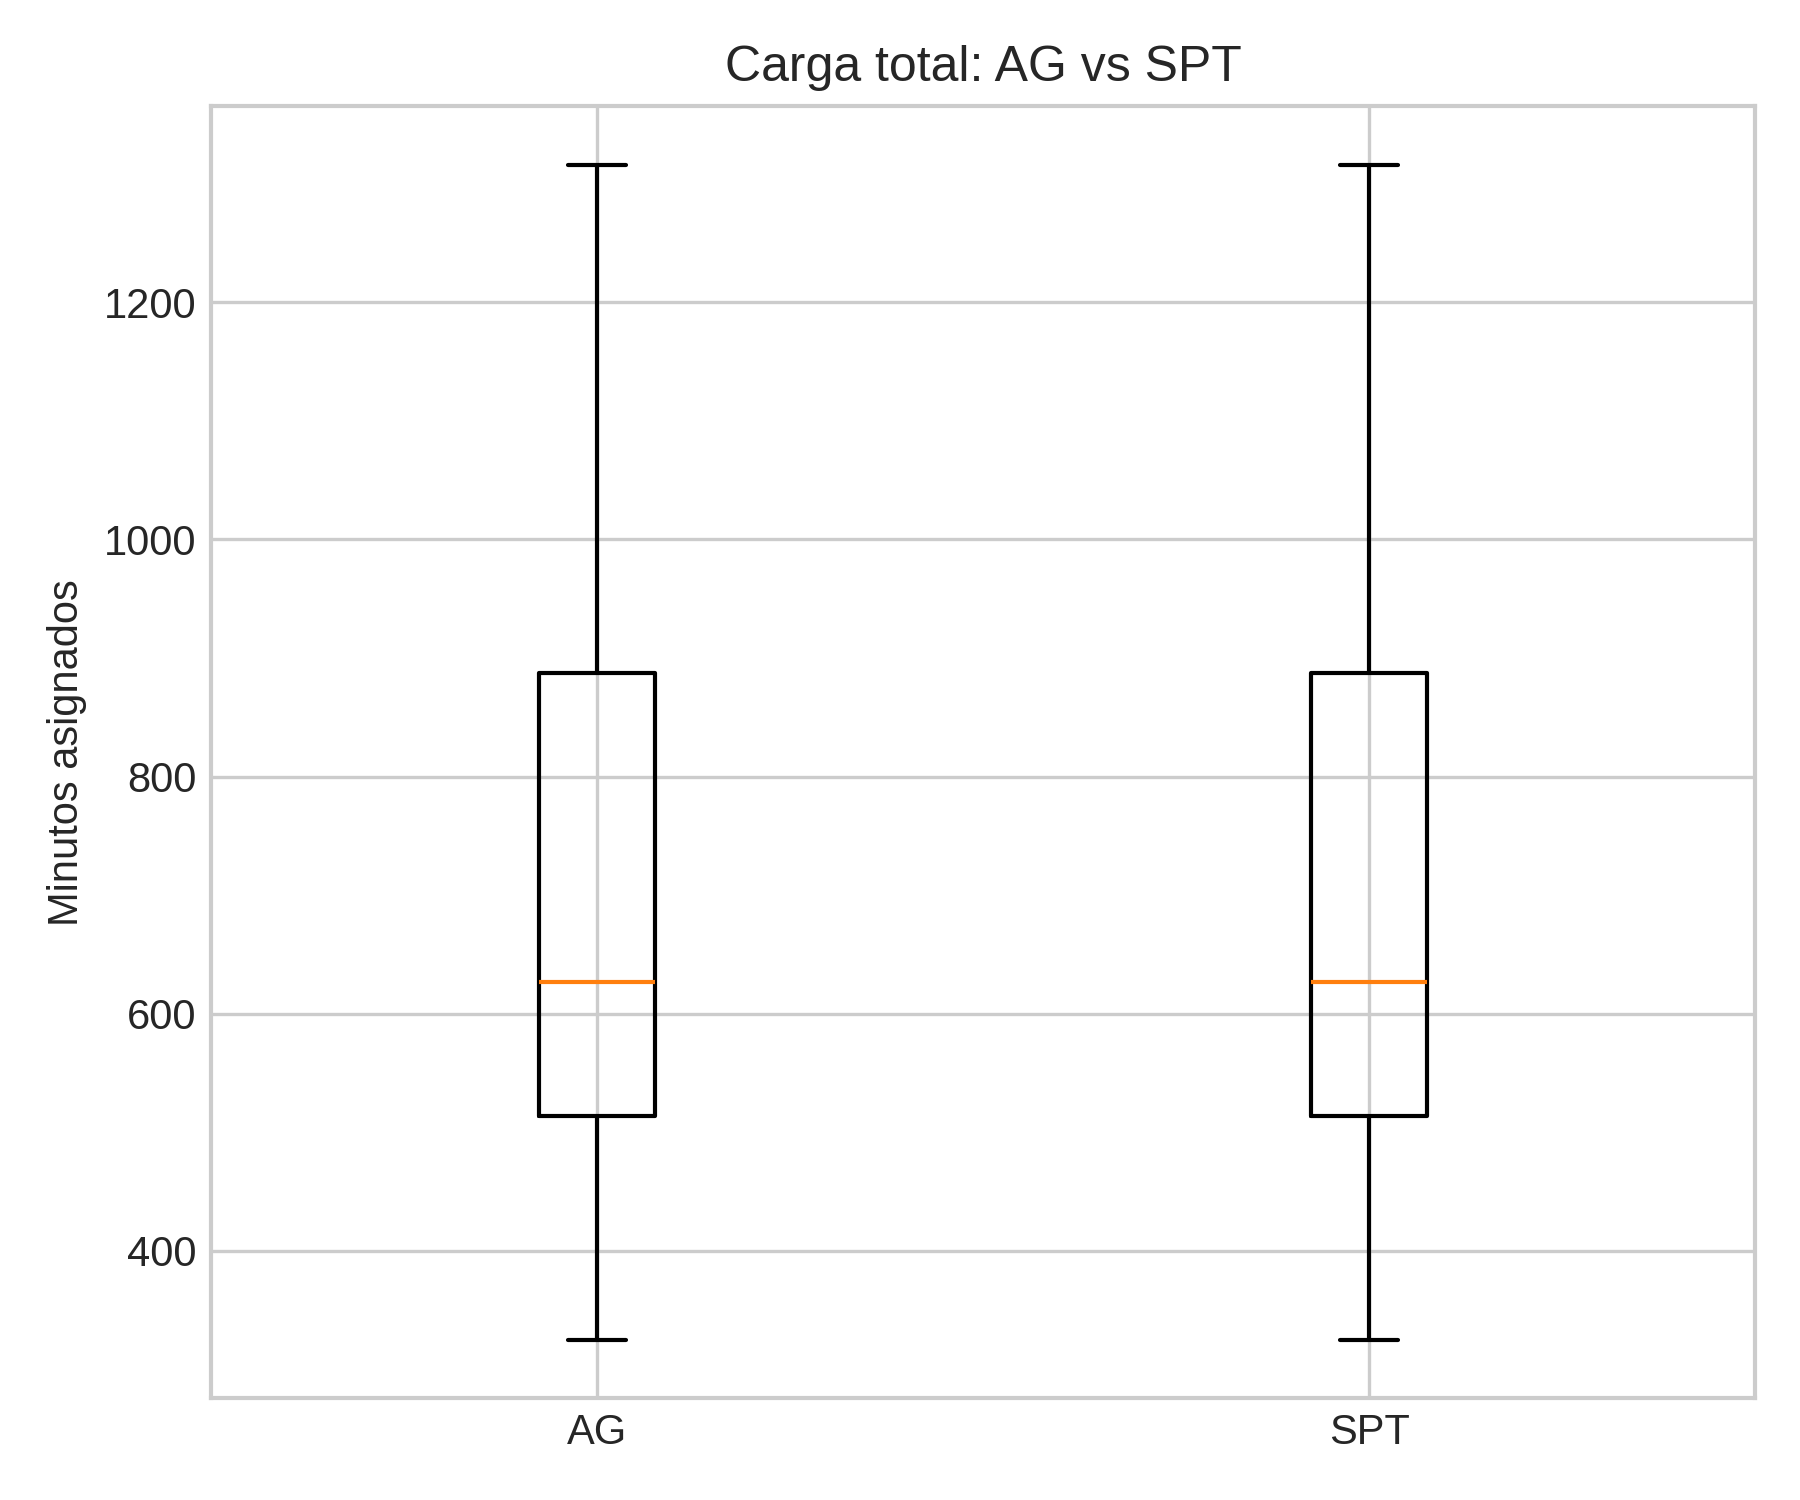
\includegraphics[width=\linewidth]{figures/carga_total.png}
    \caption{Carga total}
\end{subfigure}
\begin{subfigure}{0.45\textwidth}
    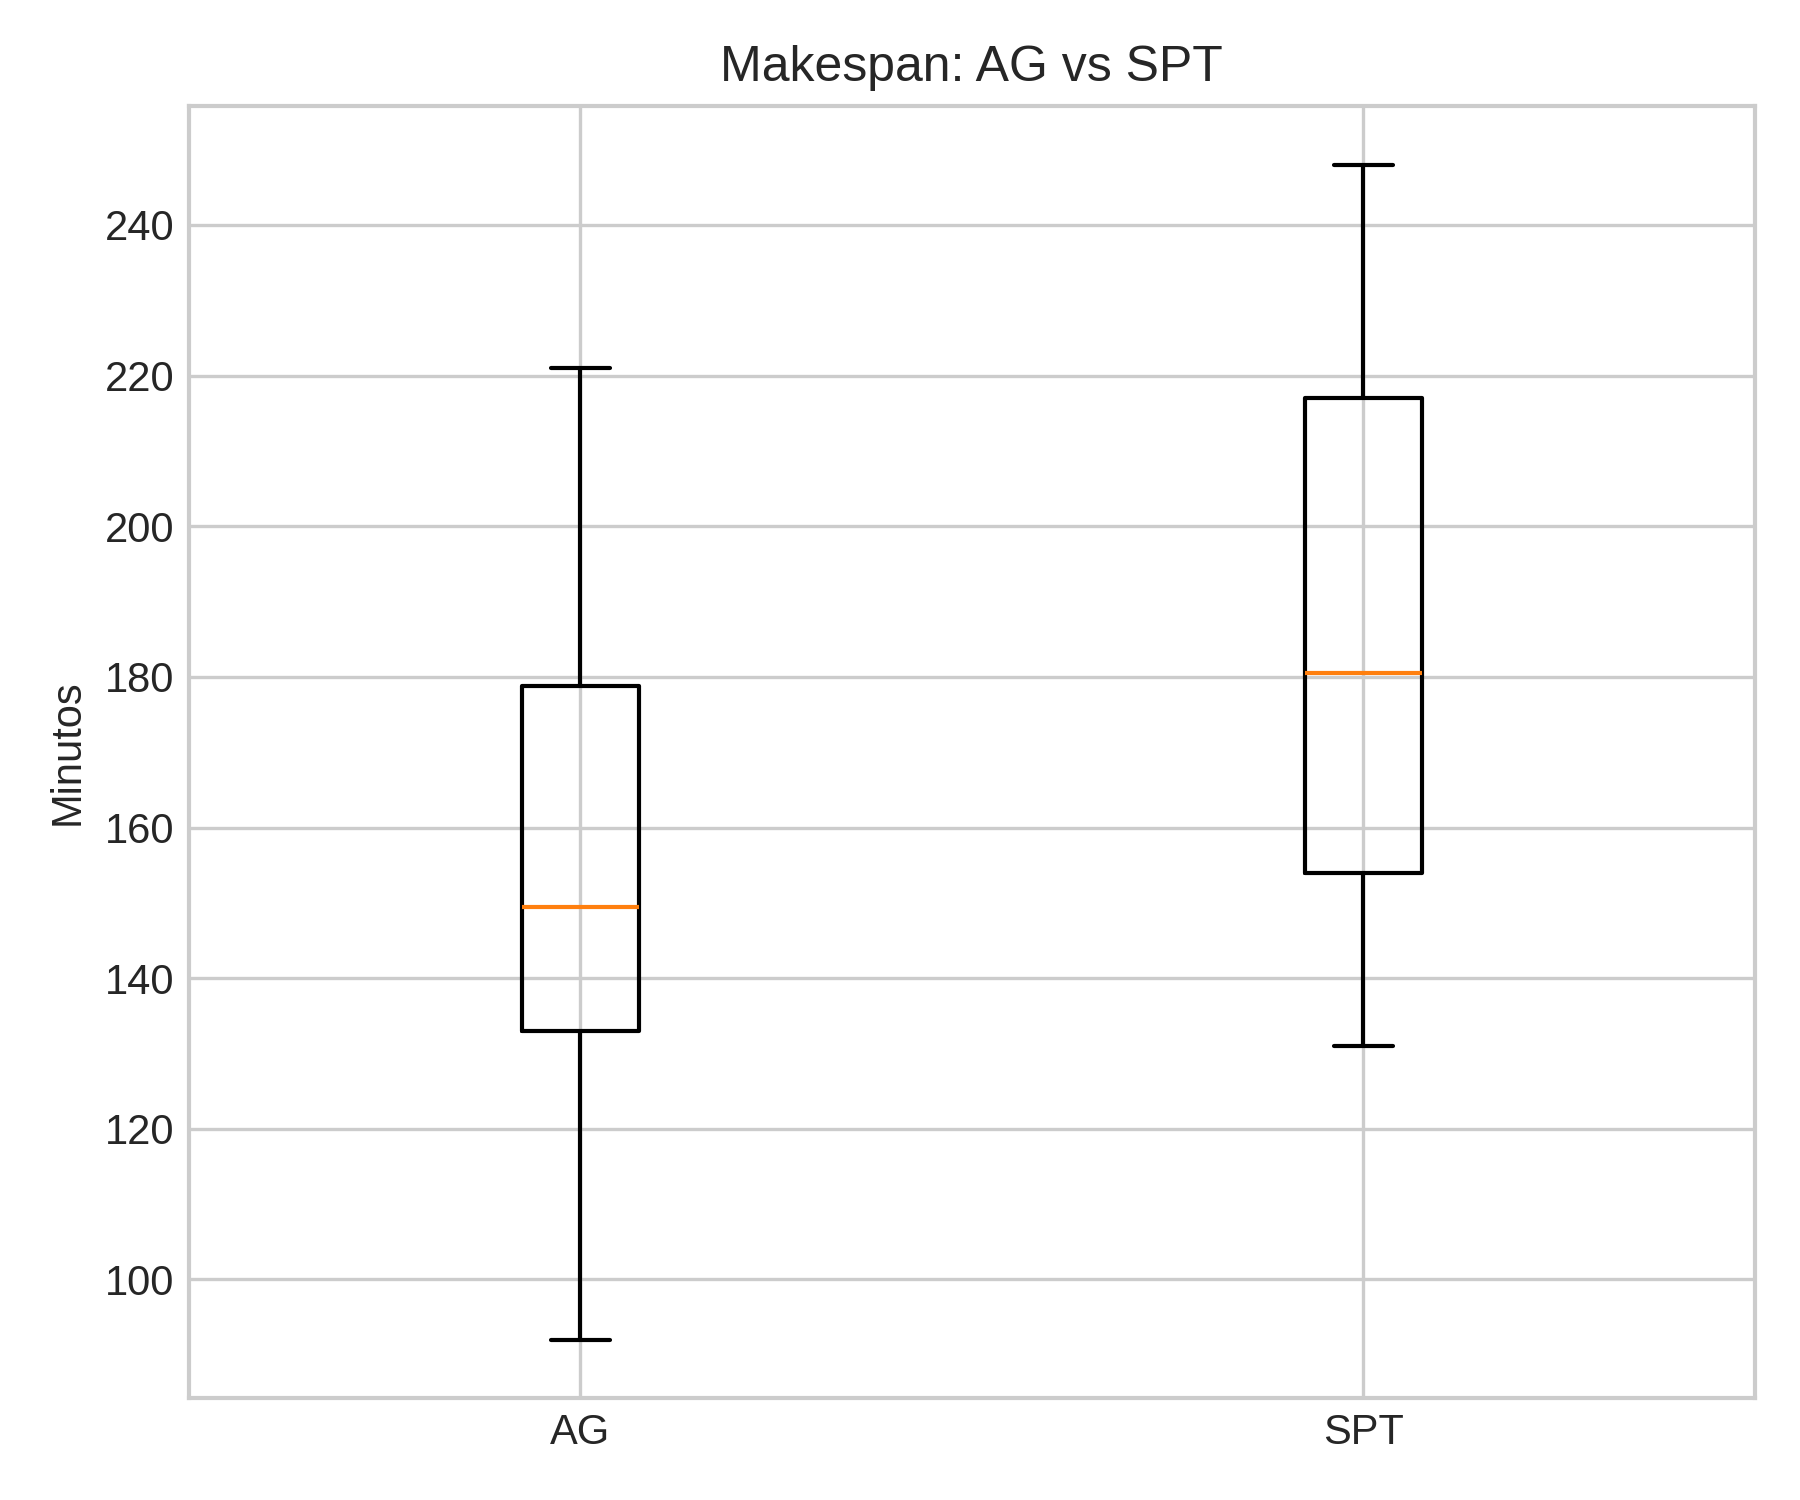
\includegraphics[width=\linewidth]{figures/makespan.png}
    \caption{Makespan}
\end{subfigure}
\caption{Uso del horizonte temporal y eficiencia global.}
\label{fig:carga-makespan}
\end{figure}

Aunque la carga total es idéntica entre algoritmos (resultado que depende directamente del número de tareas ejecutadas), el makespan del AG es mucho menor. Esto implica que el AG logra acomodar la misma cantidad de trabajo en un tiempo efectivo significativamente más corto. Industrialmente, esto se traduce en:

\begin{itemize}
    \item menor tiempo muerto entre tareas,
    \item mejores secuencias internas,
    \item menor fragmentación del trabajo,
    \item cronogramas con menos huecos entre operaciones.
\end{itemize}

El SPT, al priorizar únicamente tareas cortas, puede inducir solapamientos ineficientes o asignaciones subóptimas que extienden el makespan total.

% -------------------------------------------------------------------
\subsection{Balance entre operarios}

\begin{figure}[H]
\centering
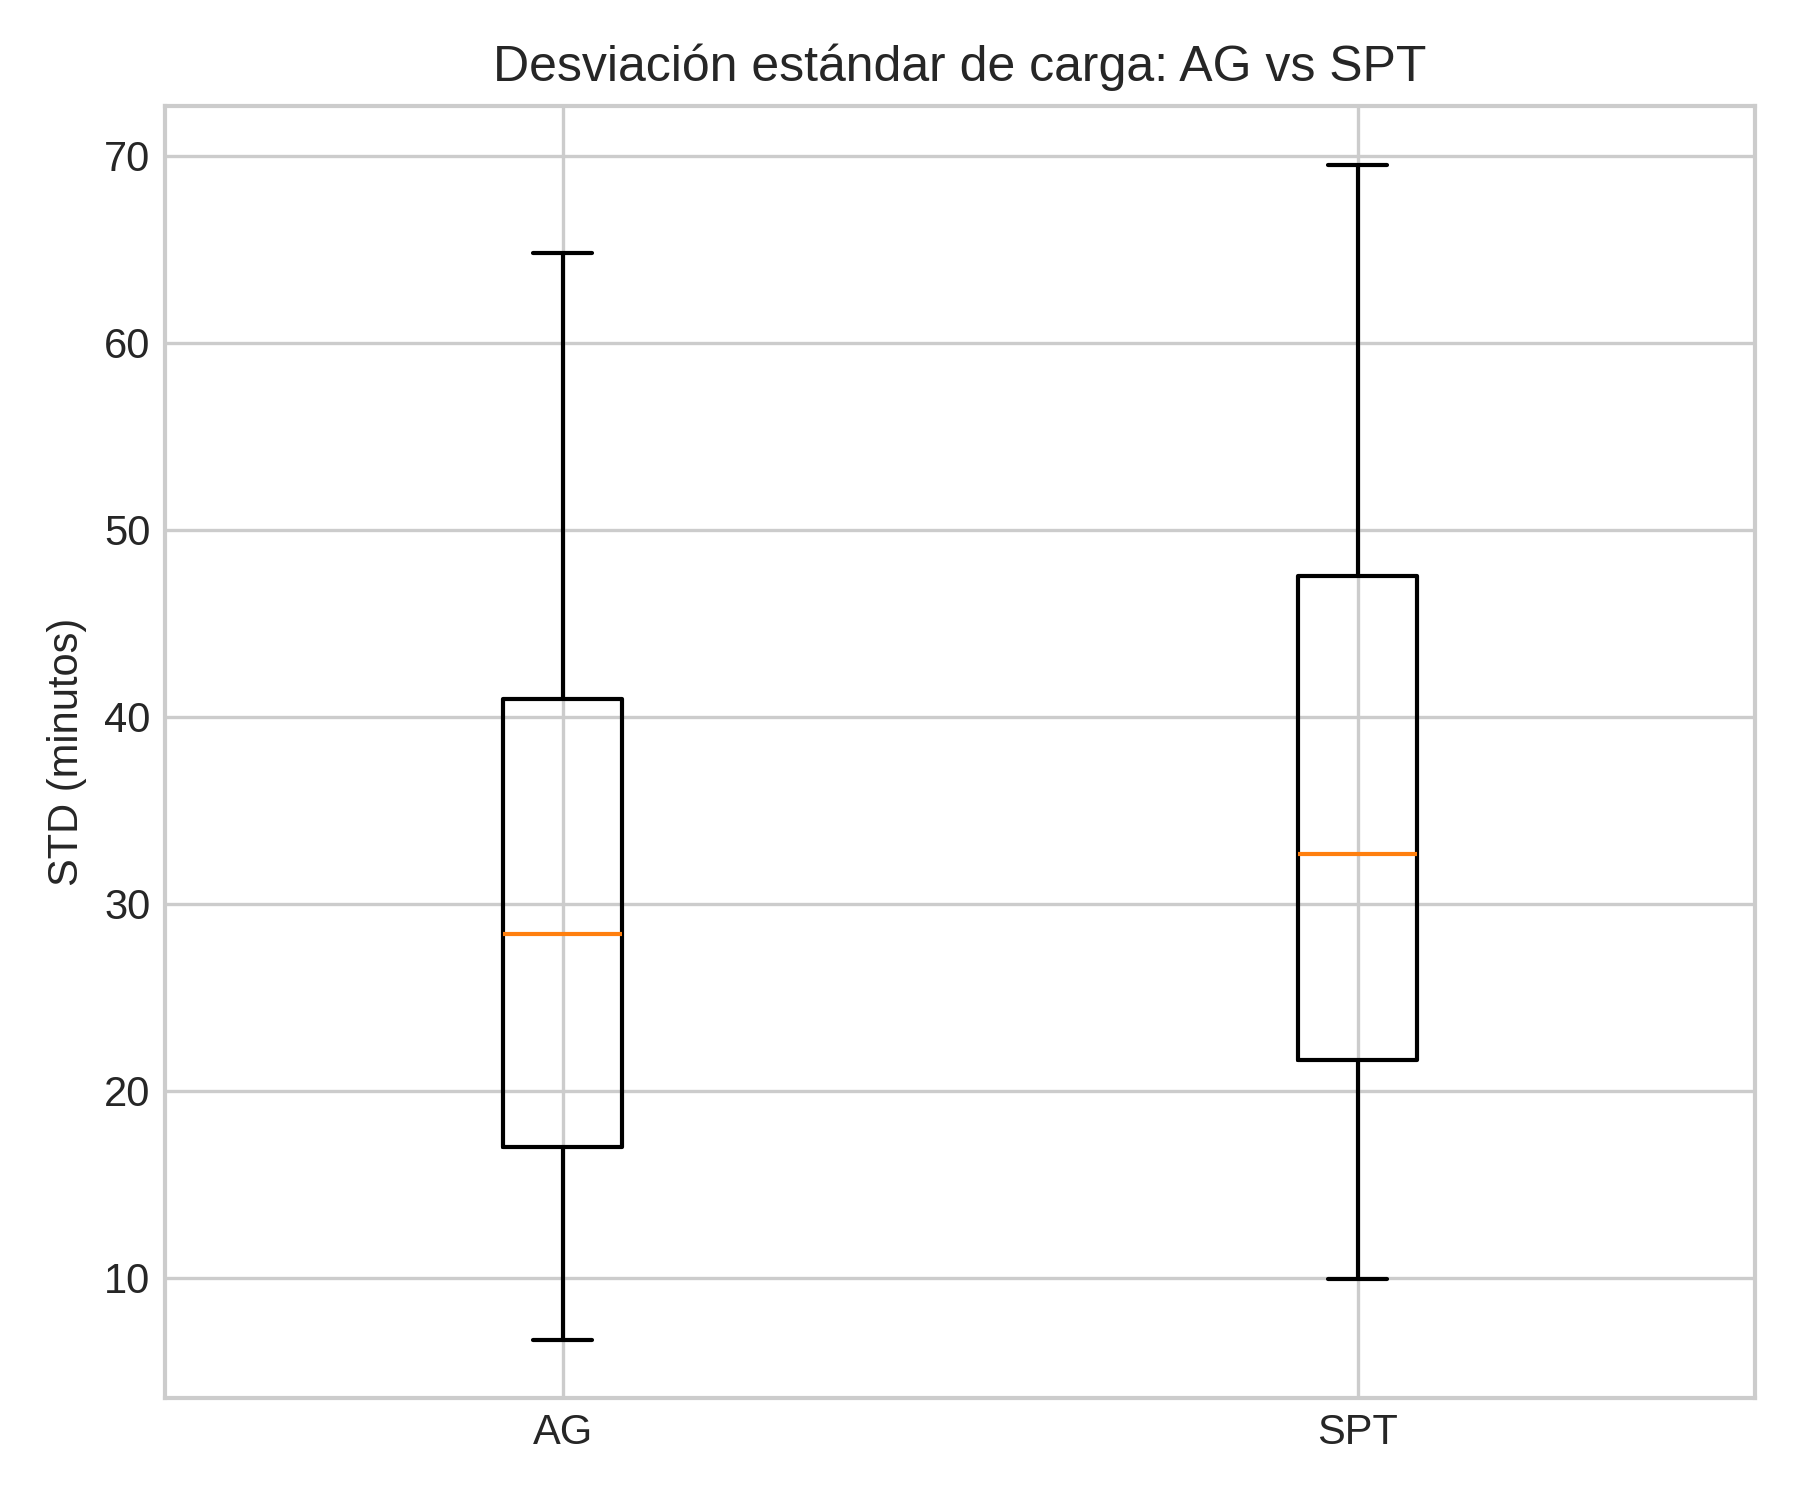
\includegraphics[width=0.55\textwidth]{figures/carga_std.png}
\caption{Desviación estándar de carga entre operarios.}
\label{fig:std-carga}
\end{figure}

El AG obtiene una desviación estándar notablemente menor, lo que indica un reparto más equilibrado del trabajo. Esta mejora no surge por casualidad, sino porque:

\begin{itemize}
    \item la función de aptitud penaliza explícitamente la mala distribución de carga,
    \item la representación del individuo codifica simultáneamente prioridades y asignación de operarios,
    \item la presión selectiva del AG favorece naturalmente soluciones más balanceadas.
\end{itemize}

Para el taller, un mejor balance significa menor riesgo de cuellos de botella, reducción de sobrecarga individual y mayor estabilidad operativa.

% -------------------------------------------------------------------
\subsection{Análisis del tiempo de ejecución}

Con el fin de cuantificar el costo computacional de ambos enfoques, se ejecutó un experimento
controlado sobre 10 instancias generadas con semilla fija (\textit{seed} = 42), cada una con
2 órdenes de trabajo. La Tabla~\ref{tab:tiempos_ejecucion} resume los estadísticos descriptivos
de los tiempos de ejecución por algoritmo.

\begin{table}[H]
\centering
\caption{Comparación de tiempos de ejecución entre AG y SPT (10 instancias, 2 OT por instancia, \textit{seed} = 42).}
\label{tab:tiempos_ejecucion}
\begin{tabular}{lccccc}
\toprule
Algoritmo & Promedio (s) & Mediana (s) & Mínimo (s) & Máximo (s) & Desv. Est. (s) \\
\midrule
AG  & 3.1284 & 2.9697 & 2.6971 & 3.7797 & 0.3907 \\
SPT & 0.000103 & 0.000103 & 0.000088 & 0.000124 & 0.0000099 \\
\bottomrule
\end{tabular}
\end{table}

Los resultados muestran que SPT presenta tiempos prácticamente instantáneos (del orden de
\(10^{-4}\) segundos), comportamiento coherente con una heurística determinística de baja complejidad.
En contraste, el AG requiere en promedio 3.13 segundos por instancia, debido a la evaluación
iterativa de poblaciones durante el proceso evolutivo (300 generaciones y 100 individuos por
población en la configuración final). Aunque este costo es mayor que el de SPT, sigue siendo
operativamente bajo para los tamaños de instancia evaluados y compatible con una planeación diaria.

% -------------------------------------------------------------------
\subsection{Ventajas y desventajas de cada enfoque}

\paragraph{Algoritmo Genético (AG):}  
\begin{itemize}
    \item \textbf{Ventajas:}
    \begin{itemize}
        \item Menor makespan.
        \item Mejor balance de carga.
        \item Mayor estabilidad entre instancias.
        \item Capacidad para capturar interacciones complejas entre precedencias, operarios y repuestos.
    \end{itemize}
    \item \textbf{Desventajas:}
    \begin{itemize}
        \item Mayor tiempo de cómputo que SPT.
        \item Requiere calibración de parámetros.
    \end{itemize}
\end{itemize}

\paragraph{SPT:}
\begin{itemize}
    \item \textbf{Ventajas:}
    \begin{itemize}
        \item Simplicidad y rapidez de ejecución.
        \item Funciona razonablemente bien en entornos con pocas restricciones internas.
    \end{itemize}
    \item \textbf{Desventajas:}
    \begin{itemize}
        \item No integra precedencias de manera natural.
        \item Puede generar secuencias ineficientes y un makespan elevado.
        \item Tiende a desequilibrar la carga entre operarios.
    \end{itemize}
\end{itemize}

% -------------------------------------------------------------------
\section{Discusión de los Hallazgos e Implicaciones}

Los experimentos demuestran que, aunque el AG y el SPT ejecutan en promedio la misma cantidad de tareas, el AG produce cronogramas significativamente más eficientes. El makespan menor y la mejor distribución del trabajo son evidencia de que el AG es capaz de capturar estructuras profundas del problema que SPT ignora debido a su simplicidad.

Desde una perspectiva industrial, esto implica:

\begin{itemize}
    \item Mayor capacidad de respuesta del taller.
    \item Horarios más compactos, que permiten atender trabajos urgentes dentro del mismo día.
    \item Menor dependencia del criterio manual o del orden de llegada.
    \item Mejor utilización del equipo humano disponible.
\end{itemize}

En conclusión, el AG no solo es competitivo frente al SPT, sino que lo supera en los aspectos más relevantes para la operación diaria del taller, justificando el uso de técnicas evolutivas en problemas reales de programación de tareas.
